\documentclass[11pt,a4paper]{article}
\usepackage[T1]{fontenc}
\usepackage[utf8]{inputenc}
\usepackage{lmodern}
\usepackage{amsmath,amssymb,amsthm,mathtools,mathrsfs}
\usepackage{graphicx,float,xcolor,multicol}
\usepackage[shortlabels]{enumitem}
\usepackage[margin=27mm]{geometry}
\usepackage{microtype,needspace,placeins}
\usepackage{tikz,tikz-cd}
\usetikzlibrary{arrows.meta,calc,positioning,patterns,decorations.pathreplacing}
\usepackage[colorlinks=true,linkcolor=teal,urlcolor=teal,citecolor=teal]{hyperref}
\setlength{\parindent}{0pt}
\setlength{\parskip}{.6em}
\setcounter{secnumdepth}{0}
\allowdisplaybreaks
\raggedbottom
\providecommand{\cross}{\times}
\DeclareUnicodeCharacter{2020}{\ensuremath{\dagger}}
\DeclareMathOperator{\supp}{supp}
\DeclareMathOperator*{\esssup}{ess\,sup}
\providecommand{\chapter}{\section}
\newenvironment{tool}[2]{\subsection*{Tool #1 --- #2}}{}
\newcommand{\ToolRef}[1]{Tool #1}
\newcommand{\FigureTag}[2]{\textit{Figure #1}}
\newcommand{\Result}[1]{\subsection*{#1}}
\newcommand{\Application}[1]{\subsubsection*{Application\if\relax\detokenize{#1}\relax\else\space--- #1\fi}}
\newcommand{\ProofHeading}{\par\textit{Proof.}\space}
\newcommand{\ProofOf}[1]{\par\textit{Proof of #1.}\space}
\newcommand{\RemarkHeading}{\par\textbf{Remark.}\space}
\newcommand{\NoteHeading}{\par\textbf{Note.}\space}
\newcommand{\ExerciseHeading}{\par\textbf{Exercise.}\space}

% Rendering support only; mathematical text is in each independent post.
\usepackage{booktabs,array,longtable}
\definecolor{HandoutBlue}{HTML}{2F6690}
\definecolor{HandoutNavy}{HTML}{17365D}
\newtheorem{theorem}{Theorem}
\newtheorem{lemma}[theorem]{Lemma}
\newtheorem{proposition}[theorem]{Proposition}
\newtheorem{corollary}[theorem]{Corollary}
\newtheorem{conjecture}[theorem]{Conjecture}
\newtheorem{definition}{Definition}
\newtheorem{example}{Example}
\newtheorem{namedtoolcounter}{Tool}
\newenvironment{namedtool}[1]{\begin{namedtoolcounter}[#1]}{\end{namedtoolcounter}}
\newtheorem*{claim}{Claim}
\newtheorem*{remark}{Remark}
\newtheorem*{exercise}{Exercise}
\newtheorem*{question}{Question}
\newtheorem*{observation}{Observation}
\newcommand{\SourceChapter}[2]{\section*{#2}}
\newcommand{\Lecture}[2]{\section*{Lecture #1: #2}}
\newcommand{\unclear}[1]{\textit{[unclear: #1]}}
\newcommand{\sourcegap}{\textit{[unfinished in the source]}}
\DeclareMathOperator{\dist}{dist}
\DeclareMathOperator{\id}{id}
\DeclareMathOperator{\Hol}{Hol}
\DeclareMathOperator{\Per}{Per}
\DeclareMathOperator{\Fix}{Fix}
\DeclareMathOperator{\diam}{diam}
\DeclareMathOperator{\Var}{Var}
\DeclareMathOperator{\Leb}{Leb}
\DeclareMathOperator{\Hom}{Hom}
\DeclareMathOperator{\End}{End}
\DeclareMathOperator{\Ann}{Ann}
\DeclareMathOperator{\Spec}{Spec}
\DeclareMathOperator{\Max}{Max}
\DeclareMathOperator{\Ob}{Ob}
\DeclareMathOperator{\Tor}{Tor}
\DeclareMathOperator{\Ass}{Ass}
\DeclareMathOperator{\Mor}{Mor}
\DeclareMathOperator{\Fun}{Fun}
\DeclareMathOperator{\Nat}{Nat}
\DeclareMathOperator{\Cone}{Cone}
\DeclareMathOperator{\MCG}{MCG}
\DeclareMathOperator{\Aut}{Aut}
\DeclareMathOperator{\Deck}{Deck}
\DeclareMathOperator{\SL}{SL}
\DeclareMathOperator{\PSL}{PSL}
\DeclareMathOperator{\Area}{Area}
\DeclareMathOperator{\im}{im}
\DeclareMathOperator{\PSh}{PSh}
\newcommand{\CRing}{\mathsf{CRings}}
\newcommand{\AMod}{A\text{-}\mathsf{Mod}}
\newcommand{\Ab}{\mathsf{Ab}}
\newcommand{\Z}{\mathbb Z}
\newcommand{\Q}{\mathbb Q}
\newcommand{\R}{\mathbb R}
\newcommand{\C}{\mathbb C}
\newcommand{\N}{\mathbb N}
\newcommand{\kk}{\mathbb k}
\renewcommand{\aa}{\mathfrak a}
\newcommand{\bb}{\mathfrak b}
\newcommand{\pp}{\mathfrak p}
\newcommand{\qq}{\mathfrak q}
\newcommand{\mm}{\mathfrak m}
\newcommand{\nn}{\mathfrak n}
\newcommand{\rad}{\mathrm r}
\newcommand{\cat}[1]{\mathsf{#1}}
\setcounter{secnumdepth}{0}
\allowdisplaybreaks

\graphicspath{{figures/lemma-book/}}
\begin{document}
\section*{Lagrange Multipliers and Boundary Analysis}
% BLOG-CONTENT-BEGIN
\subsection{Lagrange multipliers}
\setcounter{theorem}{38}\begin{lemma}[Lagrange multipliers]\label{lemma:lb1-44}
Lagrange multipliers are a powerful technique for solving constrained extremum problems.
The method uses partial derivatives.
\end{lemma}
Suppose one is given the multivariable function
$f(x,y,z)=x^2+x+2y^2+3z^2$ and $x^2+y^2+z^2=1$, and is asked to prove that
$x^2+x+2y^2+3z^2\leq25/8$.
The constant $25/8$ may look unmotivated; Lagrange multipliers reveal it naturally.
Lagrange observed that the partial derivatives of $f$ can be equated to $\lambda$ times the partial derivatives of $x^2+y^2+z^2$.
Here $\lambda$ is the Lagrange multiplier. This is like writing $\vec a=\lambda\vec b$.
\[
\frac{\partial f}{\partial x}=\lambda\frac{\partial(x^2+y^2+z^2)}{\partial x},\quad
\frac{\partial f}{\partial y}=\lambda\frac{\partial(x^2+y^2+z^2)}{\partial y},\quad
\frac{\partial f}{\partial z}=\lambda\frac{\partial(x^2+y^2+z^2)}{\partial z}.
\]
Thus we solve
\[
2x+1=2\lambda x,\qquad4y=2\lambda y,\qquad6z=2\lambda z,
\qquad x^2+y^2+z^2=1.
\]
We now have four variables and four equations. Solving them produces candidates; substituting those candidates into $f$ gives the candidate extremal values.
This statement is sometimes called Lagrange's theorem.
% Source page 15 - right
The arithmetic--geometric mean inequality provides a first example.
For positive $x,y,z$, prove that $(x+y+z)/3\geq\sqrt[3]{xyz}$.
Find the maximum of $f(x,y,z)=xyz$ with $g(x,y,z)=x+y+z=S$.
The three equations $\partial f/\partial x=\lambda\partial g/\partial x$,
$\partial f/\partial y=\lambda\partial g/\partial y$,
$\partial f/\partial z=\lambda\partial g/\partial z$ give
$yz=\lambda$, $zx=\lambda$, $xy=\lambda$.
Thus $xy=yz=zx$, so $x=y=z=S/3$. On the boundary of the nonnegative
simplex the product is zero, while at this interior point it is positive.
Plugging this into $f$ gives
\[
f(S/3,S/3,S/3)\geq f(x,y,z)
\Longrightarrow(S/3)^3\geq xyz
\Longrightarrow\frac{x+y+z}{3}\geq\sqrt[3]{xyz}.
\]
Introduce the notation ``gradient of a function $f$,'' written $\nabla f$:
\[
\nabla f(x_1,x_2,x_3)=
\left(\frac{\partial f(x_1,x_2,x_3)}{\partial x_1},
\frac{\partial f(x_1,x_2,x_3)}{\partial x_2},
\frac{\partial f(x_1,x_2,x_3)}{\partial x_3}\right).
\]

% Source page 16 - left
Instead of the first three equations in the AM--GM example, it suffices to write
$\nabla f(x,y,z)=\lambda\nabla g(x,y,z)$.
\paragraph{USAMO.}
Let $a,b,c\geq0$ and $a^2+b^2+c^2+abc=4$. Prove that $0\leq ab+bc+ca-abc\leq2$.
Put $f(a,b,c)=ab+bc+ca-abc$. We are to find its maximum and minimum under the given condition, called a constraint.
The Lagrange equations are
\[
\nabla f=\lambda\nabla(a^2+b^2+c^2+abc),
\quad (b+c-bc,a+c-ac,a+b-ab)=\lambda(2a+bc,2b+ac,2c+ab).
\]
Equivalently,
\[
\begin{cases}
b+c-bc=\lambda(2a+bc),\\
a+c-ac=\lambda(2b+ac),\\
a+b-ab=\lambda(2c+ab),\\
a^2+b^2+c^2+abc=4.
\end{cases}
\]
Solving the interior equations, together with the boundary analysis, gives
the candidates $(1,1,1)$, $(0,\sqrt2,\sqrt2)$, and their permutations.
We have $f(1,1,1)=2$ and $f(0,\sqrt2,\sqrt2)=2$.
We also notice that $(2,0,0)$ and its permutations lie on the boundary and
give $f=0$. Thus $0\leq f(a,b,c)\leq2$.

% Source page 16 - right
\paragraph{IMO (1984).}
With $x,y,z>0$ and $x+y+z=1$, prove that
$0<xy+yz+zx-2xyz\leq7/27$.
The use of Lagrange multipliers requires careful justification.
Before equating gradients, it is essential to show that the gradients are continuous.
Let $f(x,y,z)=xy+yz+zx-2xyz$ and $g(x,y,z)=x+y+z=1$.
Both are polynomials and have continuous first-order partial derivatives.
Then
\[
\nabla f=\lambda\nabla g
\Longrightarrow(y+z-2yz,x+z-2xz,x+y-2xy)=(\lambda,\lambda,\lambda).
\]
From $y+z-2yz=x+z-2xz$ we get $y-x=2z(y-x)$, so $y=x$ or $z=1/2$.
Similarly,
\[
x=y\ \text{or}\ z=\tfrac12,\qquad
y=z\ \text{or}\ x=\tfrac12,\qquad
z=x\ \text{or}\ y=\tfrac12,\qquad x+y+z=1.
\]
The interior solution is $(1/3,1/3,1/3)$. On the boundary of the closed
simplex the additional candidates are permutations of $(1/2,1/2,0)$ and
the vertices. Since $f(1/3,1/3,1/3)=7/27$, while the boundary maximum is
$1/4$ and the boundary minimum is $0$, we obtain
$0<xy+yz+zx-2xyz\leq7/27$ in the open simplex.

% Source page 17 - left
\setcounter{theorem}{39}\begin{lemma}[A warning about Lagrange multipliers]
Lagrange multipliers identify stationary candidates, but boundary and sufficiency checks remain essential.
\end{lemma}
There is a strong reason for this warning. Consider the following problem.
If $a,b,c$ are the sides of a triangle of perimeter $2$, prove that $a^2+b^2+c^2+2abc<2$.
Our constraint is $g(a,b,c)=a+b+c=2$, and we seek the maximum of
$f(a,b,c)=a^2+b^2+c^2+2abc$. The following lemma summarizes the procedure.

\setcounter{theorem}{40}\begin{lemma}[The multiplier procedure]\label{lemma:lb1-46}
In a problem where Lagrange multipliers are applied, search for a constraint on the variables.
Under this constraint, determine the extreme values of the desired function by equating the gradient of one to $\lambda$ times the gradient of the other:
$\nabla f=\lambda\nabla g$.
Then plug the solutions back into $f$ to obtain stationary candidates; boundary
and sufficiency checks are still required before identifying extrema.
\end{lemma}
For example, the preceding IMO problem gave $(1/3,1/3,1/3)$ and the
boundary candidate $(1/2,1/2,0)$. Substituting, we get $7/27$ and $1/4$;
the vertices give the boundary value $0$.
% Source page 17 - right
Lemma~\ref{lemma:lb1-46} explains the steps. Apply them now:
\[
\nabla f=\lambda\nabla g
\Longrightarrow(2(a+bc),2(b+ac),2(c+ab))=(\lambda,\lambda,\lambda).
\]
Thus $a+bc=b+ac=c+ab$, with $a+b+c=2$.
From $a+bc=b+ac$, we get $a-b=c(a-b)$, so $a=b$ or $c=1$.
Similarly, $b=c$ or $a=1$, and $c=a$ or $b=1$.
Case analysis yields $(2/3,2/3,2/3)$ and $(1,1,0)$, for which
$f(2/3,2/3,2/3)=52/27$ and $f(1,1,0)=2$.
If one incorrectly treats these candidates as the extrema, one obtains
\[
2\leq f(a,b,c)\leq52/27
\Longrightarrow2\leq a^2+b^2+c^2+2abc.
\]
This contradicts the desired inequality, so something has gone wrong. An elementary factorization reveals the missing point.
We have $a+b+c=p=2$, so $s=(a+b+c)/2=1$.
The desired inequality can be rewritten successively as
\begin{align*}
(a+b+c)^2-2(ab+bc+ac)+2abc&<2,\\
2-2(ab+bc+ac)+2abc&<0,\\
1-ab-bc-ac+abc&<0,\\
-(-1+ab+bc+ac-abc)&<0,\\
-(1-2+ab+bc+ac-abc)&<0,\\
-(1-a-b-c+ab+bc+ac-abc)&<0,\\
-(1-a)(1-b)(1-c)&<0,\\
-(s-a)(s-b)(s-c)&<0.
\end{align*}
This proves $a^2+b^2+c^2+2abc<2$.

% Source page 18 - left
The multiplier calculation overlooked the triangle inequalities. In particular, if $c=\max(a,b,c)$, then $a+b>c$.
The sides of a triangle are nonzero.
The same technique gives a variational proof of the law of reflection.
\paragraph{The law of reflection.}
\begin{figure}[H]\centering
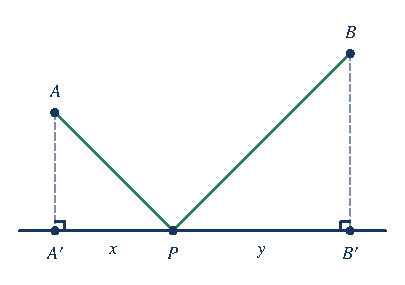
\includegraphics[width=.70\linewidth]{lb1-fig-12.pdf}
\FigureTag{LB1.12}{fig:lb1-12}
\end{figure}
It suffices to show $\angle APA'=\angle BPB'$.
We additionally use the fact that light travels along the shortest path.
The constraint is $g(x,y)=x+y=A'B'$, and $f(x,y)=AP+BP$.
Since $AP=\sqrt{x^2+(AA')^2}$ and $BP=\sqrt{y^2+(BB')^2}$,
\[
f(x,y)=\sqrt{x^2+(AA')^2}+\sqrt{y^2+(BB')^2},\qquad
\nabla f=\lambda\nabla g.
\]
Thus
\[
\left(\frac{x}{\sqrt{x^2+(AA')^2}},\frac{y}{\sqrt{y^2+(BB')^2}}\right)
=(\lambda,\lambda),\qquad
\frac{A'P}{AP}=\frac{B'P}{BP}.
\]
Also $\angle AA'P=\angle BB'P$.
% Source page 18 - right
Therefore $\triangle APA'\sim\triangle BPB'$, giving $\angle APA'=\angle BPB'$.


\paragraph{Vedant's enigma.}
Given three positive reals $x\geq y\geq z$ such that
$x^2+y^2+z^2+2xyz=1$, prove that
\[2xz+y^2\leq\frac34.\]
I asked him for a hint, to which he responded by saying that
we have $2xz=xz+xz$. I was like, ``Are you serious?!''
He makes the following threatening move:
\[2xz+y^2=xz+y^2+zx=x\cdot z+y\cdot y+z\cdot x.\]
Since $x\geq y\geq z$, we have
\[xz+yy+zx\leq\frac13(x+y+z)(x+y+z)=\frac{(x+y+z)^2}{3}.\]
Indeed,
\[
(x+y+z)^2-3(2xz+y^2)
=(x-y)^2+4(x-y)(y-z)+(y-z)^2\geq0.
\]
The constraint and positivity allow us to write
$x=\cos A$, $y=\cos B$, and $z=\cos C$, where
$A,B,C\in(0,\pi/2)$ and $A+B+C=\pi$.
Indeed, the constraint gives
$z=-xy+\sqrt{(1-x^2)(1-y^2)}=-\cos(A+B)=\cos(\pi-A-B)$.
(Don't ask me why!!)
Then
\[
\cos A+\cos B+\cos C\leq3\cos\left(\frac{A+B+C}{3}\right)
=3\cos60^\circ,
\qquad x+y+z\leq\frac32.
\]
Thus $(x+y+z)^2/3\leq\tfrac13\cdot\tfrac94=\tfrac34$, giving
$xz+y^2+zx\leq3/4$, and therefore $2xz+y^2\leq3/4$. (Q.E.D.)--1.

I gave him the following solution: ``Lagrange! Lagrange! Help!''
Let's leave it to the expert now.
Let $g(x,y,z)=x^2+y^2+z^2+2xyz=1$ be the constraint function, and maximize
$f(x,y,z)=2xz+y^2$.
The condition $\nabla f=\lambda\nabla g$ gives
\[(2z,2y,2x)=\lambda(2x+2yz,2y+2zx,2z+2xy).\]
Therefore $2z=\lambda(2x+2yz)$, $2y=\lambda(2y+2zx)$, and
$2x=\lambda(2z+2xy)$, so
\[
\frac{x+yz}{z}=\frac{y+zx}{y}=\frac{z+xy}{x}=\frac1\lambda.
\]
It follows that $x/z+y=z/x+y$, hence $z=x$.
Also $x/z+y=1+zx/y$, so $1+y=1+x^2/y$, giving $x=y$ and thus
$x=y=z=1/2$.
Consequently $(1/2,1/2,1/2)$ is the only interior stationary candidate.
The first solution supplies the global bound, and equality there forces
$x=y=z=1/2$. Hence
\[
f(x,y,z)\leq f(1/2,1/2,1/2)
=2\cdot\frac12\cdot\frac12+\frac12\cdot\frac12=\frac34.
\]
Thus $f(x,y,z)\leq3/4$, giving $2xz+y^2\leq3/4$. (Q.E.D.)--2.


\setcounter{theorem}{80}\begin{lemma}[Normalization]\label{lemma:lb1-83}
Given a homogeneous inequality, such as
\[\sum_{\mathrm{cyc}}\frac{(a+b)^2+(b+c)^2}{(a+b)(a+b+c)}>\frac{2014}{1024},\]
you can assume $a+b+c$ equals any positive number you feel like! Surprised?
\end{lemma}
Don't expect me to explain the reason for this, since we crossed these things a few pages ago.
Scaling all variables multiplies both sides of a homogeneous inequality by the same power.
\paragraph{Application.}
``What do you think? Every time I'll write applications for you? Go find one for yourself!''
$\longrightarrow$ ``Shu, shu\ldots!''
Sorry! I am not that rude; I did this just for a change.
Anyway, I have already applied this in this book. Go search!

Now let me present a surprising inequality that can be resolved using normalization.
If $x,y,z$ are real numbers, show that
\[(x^2+y^2+z^2)^3\geq(x^3+y^3+z^3)^2.\]
It is equivalent to prove
\[
\left|\sqrt[3]{x^3+y^3+z^3}\right|
\leq\sqrt{x^2+y^2+z^2}.
\]
Observe that the inequality is homogeneous.
Assume $x^2+y^2+z^2=1$, because if
$x^2+y^2+z^2=k^2$ with $k\in\mathbb R_+$, then
$(x/k)^2+(y/k)^2+(z/k)^2=1$, or $X^2+Y^2+Z^2=1$
(where $x\mapsto X$).
Now, to normalize the situation, divide by $k$:
\[
\frac{\left|\sqrt[3]{x^3+y^3+z^3}\right|}{k}
\mathrel{\stackrel{?}{\leq}}
\frac{\sqrt{x^2+y^2+z^2}}{k}.
\]
This is equivalent to
\[
\left|\sqrt[3]{\left(\frac xk\right)^3+
\left(\frac yk\right)^3+
\left(\frac zk\right)^3}\right|
\leq
\sqrt{\left(\frac xk\right)^2+
\left(\frac yk\right)^2+
\left(\frac zk\right)^2},
\]
that is, $|X^3+Y^3+Z^3|\leq1$.
It is not important to have capitals in your solution, so let
$x^2+y^2+z^2=1$.
Let us prove $|x^3+y^3+z^3|\leq1$ using Lagrange multipliers.
Set $G(x,y,z)=x^2+y^2+z^2=1$ and
$F(x,y,z)=x^3+y^3+z^3$.
Then $\nabla G=(2x,2y,2z)$ and
$\nabla F=(3x^2,3y^2,3z^2)$.
Thus $\nabla F=\lambda\nabla G$ gives
\[
\begin{aligned}
3x^2=2\lambda x&\quad\Longrightarrow\quad x=0\text{ or }x=2\lambda/3,\\
3y^2=2\lambda y&\quad\Longrightarrow\quad y=0\text{ or }y=2\lambda/3,\\
3z^2=2\lambda z&\quad\Longrightarrow\quad z=0\text{ or }z=2\lambda/3.
\end{aligned}
\]
At a stationary point, all nonzero coordinates are equal. The possible values
of $F$ are therefore
\[
\pm1,\qquad \pm\frac1{\sqrt2},\qquad \pm\frac1{\sqrt3}.
\]
Since the unit sphere is compact, $-1\leq F(x,y,z)\leq1$.
Thus $|x^3+y^3+z^3|\leq1$, and the original inequality follows. Q.E.D.!

\paragraph{A four-term AM--GM construction.}
Find the maximum value of $x(1-x^3)$ for $0\leq x\leq1$.
A four-term AM--GM estimate handles the product directly.
Let $y=x(1-x^3)$. Then $3y^3=3x^3(1-x^3)(1-x^3)(1-x^3)$.
Apply AM--GM:
\[3y^3\leq\left(\frac{3x^3+(1-x^3)+(1-x^3)+(1-x^3)}4\right)^4
=\left(\frac34\right)^4.\]
Thus $y\leq3/(4\sqrt[3]4)$; the maximum value is $3/(4\sqrt[3]4)$.
It is attained when $3x^3=1-x^3$, that is, $x=1/\sqrt[3]4$. Q.E.D.!

For comparison, the calculus solution is:
$f(x)=x-x^4$, so $f'(x)=1-4x^3=0$ gives $x=1/\sqrt[3]4$.
Thus $x=1/\sqrt[3]4$ is the only interior critical point.
We also have $f''(x)=-12x^2<0$ for $x>0$, so this point gives the maximum.
Therefore $f(1/\sqrt[3]4)=3/(4\sqrt[3]4)$.



\subsection{Boundary-analysis techniques}
To master boundary-analysis techniques, you must gather some
boundary-analysis lemmas (BALLs). I wrote two Ls because there are two
basic lemmas.
\setcounter{theorem}{85}\begin{lemma}[Boundary-analysis lemma I]\label{lemma:lb1-88}
Given a nonconstant linear function on a compact convex polytope, its maximum
and minimum are attained on the boundary.
\end{lemma}
\setcounter{theorem}{86}\begin{lemma}[Boundary-analysis lemma II]\label{lemma:lb1-89}
Given a convex function on a compact interval, its maximum is attained at an endpoint.
\end{lemma}
Now let us look at some convexity--concavity arguments that will give you
an idea of how things are done!
\paragraph{Problem 1: Romanian team selection test.}
For a given positive number $a$, find the maximum of
\[\sum_{k=1}^n(a-a_1)(a-a_2)\cdots(a-a_{k-1})a_k(a-a_{k+1})\cdots(a-a_n),\]
where $a_1,\ldots,a_n$ range independently over $[0,a]$.
Pick any one variable, say $a_k$, and consider all other $a_i$ to be constant.
You get a linear function in $a_k$, which ranges over $[0,a]$.
By Lemma~\ref{lemma:lb1-88}, the maximum is attained at an endpoint, that is, $a_k=0$ or $a$.
Argue similarly for all $a_i$. Therefore the sum reaches its maximum for a certain choice of $a_k=0$ or $a$, $k=1,\ldots,n$.
% Source page 47 - right
If all $a_k=0$, the sum is zero. If two or more $a_k=a$, the sum is zero.
If one $a_k=a$ and the others are zero, the sum is $a^n$.
Thus the maximum value is $a^n$.
\paragraph{Problem 2: Titu Andreescu.}
Let $0\leq a,b,c,d\leq1$. Prove that
\[(1-a)(1-b)(1-c)(1-d)+a+b+c+d\geq1.\]
Choose any one variable and let the others be constant.
It is a linear function, so it attains its minimum when the chosen variable is either zero or one.
Argue similarly for all four variables, giving $(a,b,c,d)=0$ or $1$.
At a Boolean vertex, the value is $1$ when all four variables are zero, and
otherwise it is the number of variables equal to one.
We observe that $1$ is the smallest of all the values obtained, so the minimum of the function is $1$.
The conclusion follows.
These are some standard techniques, but there are one or two more problems with quite a different way of sorting things.
\paragraph{Problem 3: W. L. Putnam Mathematical Competition.}
Let $n$ be a natural number and $x_i\in[0,1]$ for $i=1,2,\ldots,n$.
Find the maximum of $\sum_{i<j}|x_i-x_j|$.
% Source page 48 - left
Applying the endpoint argument successively shows that the maximum is attained when every $x_i$ equals zero or one.
Let $p$ of them be zero and $n-p$ of them be one.
Then the sum is $p(n-p)$, whose maximum over integral $p$ is $\lfloor n^2/4\rfloor$.
\paragraph{Problem 4: USAMO.}
If $a,b,c,d,e\in[p,q]$ with $p>0$, prove that
\[(a+b+c+d+e)\left(\frac1a+\frac1b+\frac1c+\frac1d+\frac1e\right)
\leq25+6\left(\sqrt{\frac pq}-\sqrt{\frac qp}\right)^2.\]
Fix $a,b,c,d$ to be constants. The left-hand side is now of the form
$\widehat a x+\widehat b/x+\widehat c$, where $\widehat a,\widehat b,\widehat c>0$ and $x\in[p,q]$.
This is a convex function, so it attains its maximum at an endpoint.
Thus each of $a,b,c,d,e$ is either $p$ or $q$.
If $n$ of them equal $p$ and $5-n$ equal $q$, then the left-hand side has the form
\[n^2+(5-n)^2+n(5-n)\left(\frac pq+\frac qp\right)
=25+n(5-n)\left(\sqrt{\frac pq}-\sqrt{\frac qp}\right)^2.\]
This completes the endpoint argument.
So now you have two bats and two balls. What are you waiting for?
Go play with some problems and enjoy yourself.
Okay, I'll give you problems to throw away\ldots\ here they come!
% Source page 48 - right
\paragraph{Problem 1.}
The nonnegative numbers $a,b,c,A,B,C,k$ satisfy $a+A=b+B=c+C=k$.
Prove that $aB+bC+cA\leq k^2$.
\paragraph{Problem 2.}
Prove that for $a,b,c\in[0,1]$,
\[\frac a{b+c+1}+\frac b{c+a+1}+\frac c{a+b+1}+(1-a)(1-b)(1-c)\leq1.\]
\paragraph{Problem 3.}
Prove that if $1\leq x_k\leq2$ for all $k=1,2,\ldots,n$, then
\[\left(\sum_{k=1}^n x_k\right)\left(\sum_{k=1}^n\frac1{x_k}\right)^2\leq n^3.\]
The third is more difficult; here is a solution.
\[\sqrt[3]{\left(\sum_{k=1}^n x_k\right)\left(\sum_{k=1}^n\frac1{x_k}\right)^2}
\leq\frac13\left(\sum_{k=1}^n x_k+\sum_{k=1}^n\frac1{x_k}+\sum_{k=1}^n\frac1{x_k}\right)
=\sum_{k=1}^n\frac{x_k+2/x_k}{3}.\]
The function $x+2/x$ is convex, with its maximum at an endpoint of the interval, that is, $x_k=1$ or $2$.
In both cases we end up with $3$, so $(x_k+2/x_k)/3\leq1$.
Thus $\sum_{k=1}^n(x_k+2/x_k)/3\leq n$.
This proves the claim.


Coordinate methods can also help with extremal questions about the area of a triangle.
\setcounter{theorem}{101}\begin{lemma}[Hadamard's inequality]
If $A=(a_{ij})$ is an $n\times n$ matrix, then
$|\det A|^2\leq\prod_{i=1}^n\bigl(\sum_{j=1}^n|a_{ij}|^2\bigr)$.
If no row is zero, equality holds if and only if the rows are pairwise
orthogonal. A zero row also gives equality.
\end{lemma}
\paragraph{Application: Mathematical Reflections, issue 1 (2014).}
In triangle $ABC$, a point $P$ is at distances $R_1=1$, $R_2=2$, $R_3=3$ from $A,B,C$.
Find the maximum area of $ABC$.
Place $P$ at the origin, with $A=(x_1,y_1)$, $B=(x_2,y_2)$, $C=(x_3,y_3)$.
Then $x_i^2+y_i^2=R_i^2$ and
\[
[ABC]=\frac12\begin{vmatrix}1&x_1&y_1\\1&x_2&y_2\\1&x_3&y_3\end{vmatrix},\qquad
\begin{vmatrix}1&x_1&y_1\\1&x_2&y_2\\1&x_3&y_3\end{vmatrix}^{\!2}
\leq(R_1^2+1)(R_2^2+1)(R_3^2+1).
\]
The determinant estimate gives
\[
[ABC]\leq\frac12\sqrt{(R_1^2+1)(R_2^2+1)(R_3^2+1)}.
\]
This gives $[ABC]\leq5$, but equality would require the three rows to be
orthogonal, which is impossible here. We therefore finish the maximization.
After a rotation and, if needed, a reflection, put
\[
A=(1,0),\qquad B=2(\cos\beta,\sin\beta),\qquad
C=3(\cos\gamma,\sin\gamma),\qquad 0\leq\beta\leq\pi.
\]
Twice the area is
\[
2[ABC]=2\sin\beta+6\sin(\gamma-\beta)-3\sin\gamma.
\]
For fixed $\beta$, maximize over $\gamma$. Writing $c=\cos\beta$, we get
\[
2[ABC]\leq2\sqrt{1-c^2}+3\sqrt{5-4c}=:F(c),qquad -1\leq c\leq1,
\]
and the choice of $\gamma$ giving equality is available. The unique critical
point of $F$ in $(-1,0)$ is the negative root $c_0$ of
\[
4c^3-14c^2+9=0.
\]
The derivative is negative on $(0,1)$, and comparison with the endpoints
shows that this critical point gives the maximum. Therefore
\[
\max[ABC]=\sqrt{1-c_0^2}+\frac32\sqrt{5-4c_0}
\approx4.904822,
\qquad c_0\approx-0.729379.
\]

% Source page 11 - left
% BLOG-CONTENT-END
\end{document}
